
An overview of \toolName\ is depicted in Fig.~\ref{fig:overview}.
\toolName\ takes as input the models for the robots (\circled{1}) and of the environment in which they are deployed (\circled{2}) and the mission each robot should achieve (\circled{3}).
Both the models of the robots and their environment may be partial since there can be uncertainty about information contained in these models.
\toolName\ uses the model of the environment and the robots to compute plans that allow to achieve missions using an appropriate planner.
The implemented planner is able to compute plans that definitely ensure the mission satisfaction, i.e., definitive plans  (\circled{4}), and plans that may ensure property satisfaction since they depend on some partial knowledge present in the models of the robots and the environment  (\circled{5}).
More precisely, a \emph{definitive plan} is a sequence of actions that ensure the satisfaction of the local mission for each robot. 
A \emph{possible plan} is a sequence of actions that may satisfy the local mission due to some unknown information about the model of the robots or the environment in which they are deployed. 
If \toolName\ is not able to find neither a definitive nor a possible plan a message is sent to the user (\circled{6}).
Otherwise, an appropriate component is used to choose between definitive and possible plans (if both are present) or simply chooses the possible plan if no definitive plan is present.
Definitive plans are not present when the only way to satisfy the local mission is based on some unknown information about the model of the robots or the environment in which they are deployed. 
\toolName\ then executes the selected plan (\circled{7}).

As robots perform plans, information about uncertain parts of the model is detected.
\toolName\ updates the  models with the detected information (\circled{8}).
If \toolName\  detects that a plan is not anymore executable, the planner is re-executed (\circled{9}).




In the following, we provide some additional information about the inputs processed  by \toolName, the planning algorithm, the selection between definitive and possible plans and how models are updated when information about uncertain parts is detected.




\textbf{Models of the robots and their environment}. 
The models of the robots and their environments are provided using a specific form of transition system that allows the specification of uncertain parts that is described  in~\cite{mapmaker17}.
These models describe the initial positions of the robots, the map that describes the environment where robots are deployed and how robots can move between different locations of the map. 
Furthermore, the proposed models embed partial knowledge as follows:\\
%\textbf{Uncertainties supported by \toolName}.
$\bullet$  \emph{Partial knowledge about the actions' execution.} 
The execution of certain action is uncertain meaning that it is unclear whether the action can be executed.
This type of partial knowledge allows specifying that the transition between two of the cells that form the grid map of the environment can be:
always possible, always not possible (i.e. a wall), not known (i.e. a door between two rooms that can be open or closed).\\
$\bullet$ \emph{Unknown service provisioning.} 
It is unclear  whether a service can be provided or not in a specific location. 
For example, it is unclear whether a robot can take a picture of an item in a given map location.
This  uncertainty may be caused for example by the presence of an unexpected object that covers the robot visual in that location.\\
$\bullet$ \emph{Unknown meeting capabilities.} Robots can meet and synchronize in certain locations.
For example, it is unclear whether two robots can exchange a load in a given map location.
This uncertainty may be caused by a collapsing registered in the environment where the robots are deployed.


\begin{figure}[t]
\begin{center}
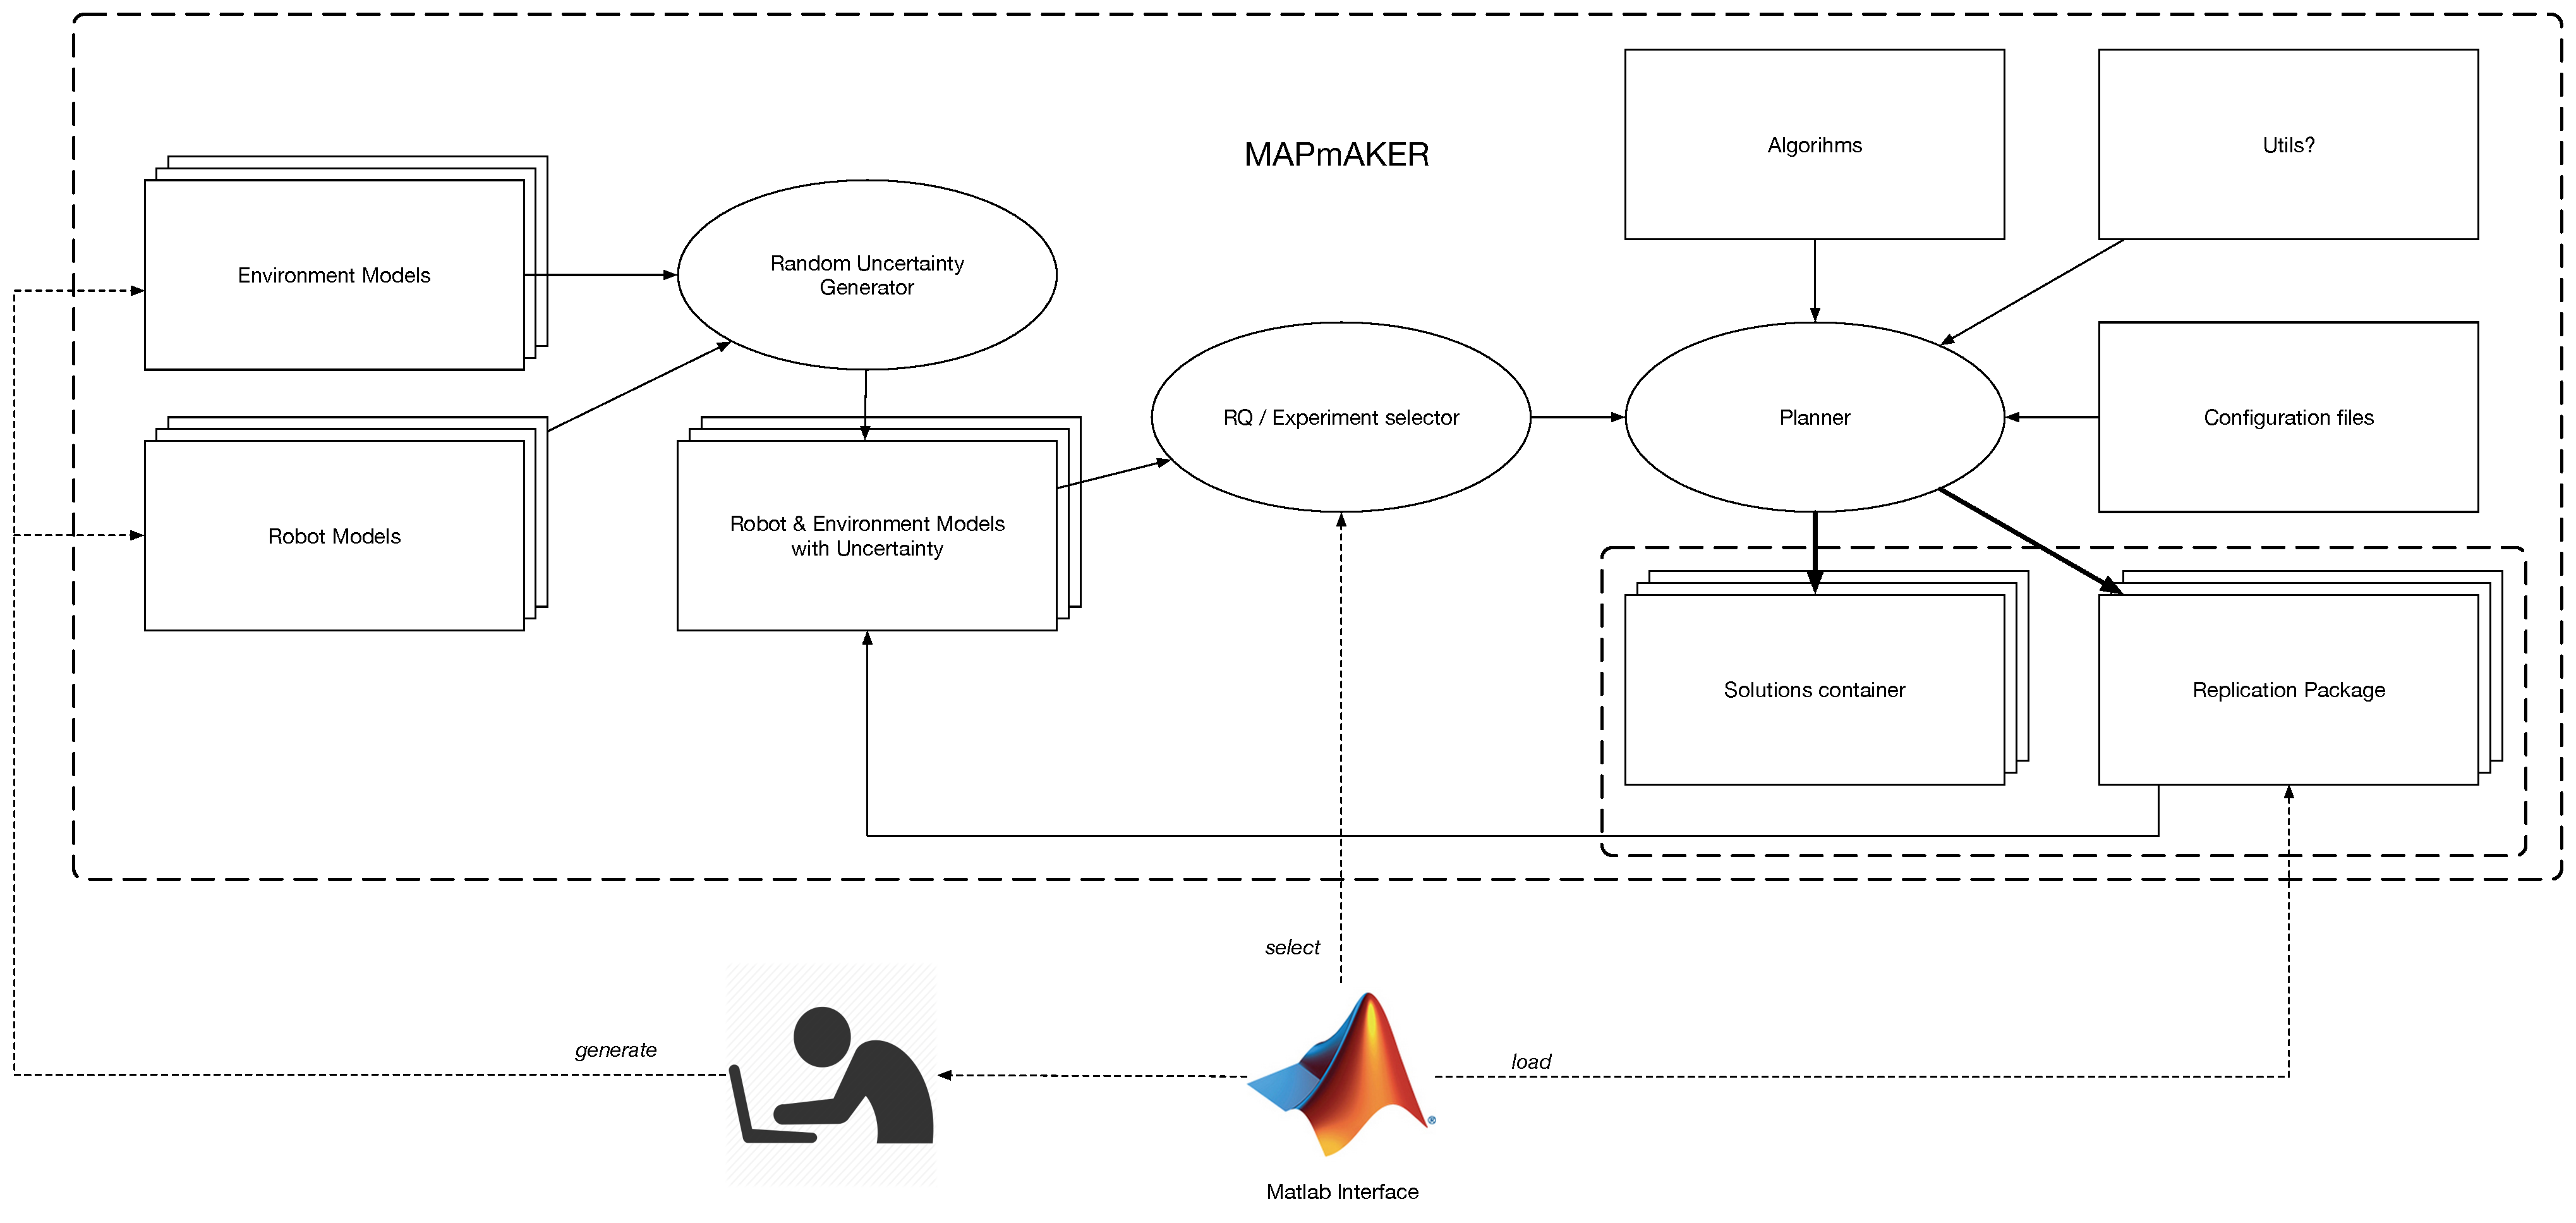
\includegraphics[width=1\linewidth]{Figures/MAPmAKER.pdf}
\caption{Overview of  MAPmAKER.}
\label{fig:overview}
\end{center}
\end{figure}




\textbf{Mission specification.}
Each robot is able to perform a complex mission, which is specified using an LTL formula.
This formula specifies how the services must be provided by the robots.
For example, a mission for a robot $r_1$ may require $r_1$ to  periodically load debris on $r_2$.
Thus, in order to allow robot $r_1$ to fulfill its mission it is necessary that robots $r_1$ and $r_2$ synchronize their behaviours.





\textbf{Planning.} 
The \emph{Planner}  uses the models of the robot(s) and the environment in order to compute plans that allow satisfying the missions of the robots.
The planner decomposes the robots within the robotic application into dependency classes based on the mission that each robot has to achieve.
Each dependency class contains a subset of robots that depend on each other for achieving their missions.
After  dependency classes are computed they are considered in isolation regarding the computation of plans that allow robots to satisfy their missions.

To compute a plan for a dependency class the  LTL formulae that are used to describe missions are evaluated on partial models.
Possible and definitive plans are computed by executing a classical planning algorithm twice: once for computing possible plans and once for computing definitive plans.
%The proposed algorithm There exists a subset of LTL formulae, known in literature as self-minimizing formulae



\textbf{Choosing between definitive and possible plans.}
The plan selector component aims at choosing between possible and definitive plans.
%The tool always try to reach the goal performing the lower number of actions.
%This work does not discuss how to choose between
%37 possible and de nitive plans. 
Several policies can be applied to choose between these plans.
Possible plans can be chosen only in cases in which a definitive plan is  not present.
Another policy may choose the plan with the shortest length, or it may consider non-functional aspects of the plans e.g., time to perform certain actions, or likelihood of detecting true or false evidence about partial information. 
In this work we assume  that the planner always chooses the shortest between the possible and the definitive plan.
This policy may, for example, reduce energy consumption, since every action performed by the robots may consume energy. 
%Thus, shorter plans require less energy.

\textbf{Detection of uncertain information.}
As robots perform actions and navigate within the environment, information regarding uncertain actions services and meeting capabilities can be detected.
Specifically, robots detect whether actions, services and meeting capabilities are executable, provided, and possible, respectively.
\toolName\ updates the models of the robots and of the environment with the detected information.
Then, if needed, the planning algorithm is triggered and re-executed.
%This information is shared with the rest of the team so it can be take into account for further planning.






